
% Preamble
\documentclass[11pt]{article}

% Packages
\usepackage{amsmath}
\usepackage{mathtools}
\usepackage{ragged2e}
\usepackage [utf8]{inputenc}
\usepackage{blindtext}
\usepackage{wrapfig}
\usepackage{xcolor}
\usepackage {polski}
\usepackage{multicol}
\usepackage[a4paper, total={5.7in, 8in}]{geometry}
\usepackage{graphicx}
\usepackage{amstex}
\usepackage{csvsimple}
\usepackage{changepage}
\usepackage{enumitem}
\usepackage[english]{babel}
\usepackage{biblatex}
\usepackage{caption}
\usepackage{indentfirst}
\usepackage{epstopdf-base}

% Document
\begin{document}
%    Nagłówek
    \begin{flushleft}
        Filip Krauz-Damski 267 681 \hfill Data wykonania ćwiczenia:\\
        Filip Kubecki 272 655 \hfill 29 kwietnia 2024r\\
        \hfill Data sporządzenia sprawozdania:\\
        Grupa: Pon 13:15 \hfill 5 maja 2024r\\
    \end{flushleft}
    \begin{center}
        \Large\textbf{Ćwiczenie 7.}\\
        \textbf{Pomiary mocy, wyznaczanie sprawności odbiornika}
    \end{center}
    \vspace{2cm}
%    Treść
    \section{Spis przyrządów}
    \par{
        Do wykonania ćwiczenia wykorzystano:
        \begin{itemize}
            \setlength\itemsep{0em}
            \item[-] Miernik zużycia energii e246
            \item[-] Miernik portu USB Keweisi KWS-V20
            \item[-] Zasilacz laboratoryjny symetryczny NDN DF1730SL20A
        \end{itemize}
    }

    \section{Przebieg i cele doświadczenia}
    Doświadczenie polegało kolejno na:
    \begin{itemize}
        \setlength\itemsep{0em}
        \item Rejestrowaniu prądu i współczynnika mocy na wejściu ładowarki ładującej kolejno 3 różne urządzenia oraz rejestrowaniu napięcia i natężenia prądu na wyjściu ładowarki,
        \item Rejestrowaniu mocy na wejściu zasilacza laboratoryjnego oraz napięcia i natężenia na wyjściu zasilacza
        obciążone przez rezystor HS50,
        \item Pomiaru mocy i współczynnika mocy urządzeń przekazanych przez prowadzącego,
    \end{itemize}
    \newpage
    \section{Wyniki pomiarów}
    \subsection*{Część 1 - Pomiar mocy ładowanych urządzeń}
    \begin{center}
    \textbf{\small Tabela 1 - Smartphone Realme}
    \end{center}
    \begin{center}
        \csvreader[tabular = |c|c|c|c|c|,
            table head = \hline  \textbf{T[min]} & \textbf{\boldmath$I_{ac}$[A]} & \textbf{PF} & \textbf{\boldmath$I_{dc}$[A]} & \textbf{\boldmath$U_{dx}$[V]}  \\\hline,
            late after line = \\\hline
        ]{Dane/Dane1.csv}{}{
            \csvcoli & \csvcolii & \csvcoliii & \csvcoliv & \csvcolv
        }
    \end{center}
    Poziom naładowania przed doświadczeniem: 74[\%].\\
    Poziom naładowania po doświadczeniu: 88[\%].
    \newpage
    \begin{center}
        \textbf{\small Tabela 2 - Smartphone OnePlus}
    \end{center}
    \begin{center}
        \csvreader[tabular = |c|c|c|c|c|,
            table head = \hline  \textbf{T[min]} & \textbf{\boldmath$I_{ac}$[A]} & \textbf{PF} & \textbf{\boldmath$I_{dc}$[A]} & \textbf{\boldmath$U_{dx}$[V]}  \\\hline,
            late after line = \\\hline
        ]{Dane/Dane2.csv}{}{
            \csvcoli & \csvcolii & \csvcoliii & \csvcoliv & \csvcolv
        }
    \end{center}
    Poziom naładowania przed doświadczeniem: 81[\%].\\
    Poziom naładowania po doświadczeniu: 90[\%].
    \newpage
    \begin{center}
        \textbf{\small Tabela 3 - Opaska sportowa}
    \end{center}
    \begin{center}
        \csvreader[tabular = |c|c|c|c|c|,
            table head = \hline  \textbf{T[min]} & \textbf{\boldmath$I_{ac}$[A]} & \textbf{PF} & \textbf{\boldmath$I_{dc}$[A]} & \textbf{\boldmath$U_{dx}$[V]}  \\\hline,
            late after line = \\\hline
        ]{Dane/Dane3.csv}{}{
            \csvcoli & \csvcolii & \csvcoliii & \csvcoliv & \csvcolv
        }
    \end{center}
    Poziom naładowania przed doświadczeniem: 5[\%].\\
    Poziom naładowania po doświadczeniu: 31[\%].

    \subsection*{Część 2 - Pomiar mocy zasilacza labolatoryjnego}
    \begin{center}
        \textbf{\small Tabela 4}
    \end{center}
    \begin{center}
        \csvreader[tabular = |c|c|c|c|,
            table head = \hline  \textbf{U[V]} & \textbf{I[A]} & \textbf{P[W]} & \textbf{PF}  \\\hline,
            late after line = \\\hline
        ]{Dane/Dane4.csv}{}{
            \csvcoli & \csvcolii & \csvcoliii & \csvcoliv
        }
    \end{center}

    \subsection*{Część 3 - Pomiar mocy urządzeń przekazanych przez prowadzącego}
    \begin{center}
        \textbf{\small Tabela 5}
    \end{center}
    \begin{center}
        \csvreader[tabular = |c|c|c|,
            table head = \hline  \textbf{Urządzenie} & \textbf{Moc[W]} & \textbf{PF}  \\\hline,
            late after line = \\\hline
        ]{Dane/Dane5.csv}{}{
            \csvcoli & \csvcolii & \csvcoliii
        }
    \end{center}

    \section{Analiza wyników}
    \subsection*{Część 1 - pobór energii}
    \textbf{Uwaga!} - napięcie sieciowe zmierzone na początku zadania wynosiło około 240[V]. Takie napięcie będzie wykorzystywane więc w obliczeniach.\\
    \indent Z powodu zaniedbania eksperymentatorów nie zostało również odnotowane wskazanie energii pobrane w ciągu ładowania przez urządzenia. W analizie danych
    zostanie użyta więc tylko energia wynikająca z obliczeń. \\
    \indent Dodatkowo dla ładowania opaski sportowej miernik nie wskazywał wartości współczynnika mocy.
    Mogło to być spowodowane bardzo małym poborem mocy przez ładowarkę tego urządzenia. Jako że ładowartka tego urządzenia jest bardzo podobna
    do ładowarki poprzednich 2 urządzeń, za współczynnik mocy uznano średnią wartość współczynnika mocy dla wszystkich poprzednich pomiarów. Współczynnik
    mocy dla pomiaru poboru energii opaski zastosowany w obliczeniach będzie wynosił więc 0.5.\\
    \\
    \noindent Moc czynna dla pradu zmiennego sieciowego zostałą wyznaczona ze wzoru:
    \begin{gather*}
        P=I\cdot U\cdot \cos(\varphi)=I\cdot U\cdot PF
    \end{gather*}
    \noindent Przykładowo dla urządzenia Realme w piątej minucie eksperymentu:
    \begin{gather*}
        P=0.082[A]\cdot 240 [V]\cdot 0.56\approx 11.021[W]
    \end{gather*}
    \noindent Moc prądu stałego na wyjściu ładowarki obliczono ze wzoru:
    \begin{gather*}
        P=I\cdot U
    \end{gather*}
    \noindent Przykładowo dla urządzenia Realme w piątej minucie eksperymentu:
    \begin{gather*}
        P=1.05[A]\cdot 9.4[V]\approx 9.870[W]
    \end{gather*}
    \newpage
    \par Energię pobraną do naładowania urządzenia z obu mierników wyznaczono licząc całkę mocy czynnej w czasie. Obliczenie zostało wykonane przy pomocy
    oprogramowania OriginPro. Poniżej przedstawiono przykładowy wykres oraz wyniki kalkulacji oprogramowania dla urządzenia Realme:
    \begin{center}
        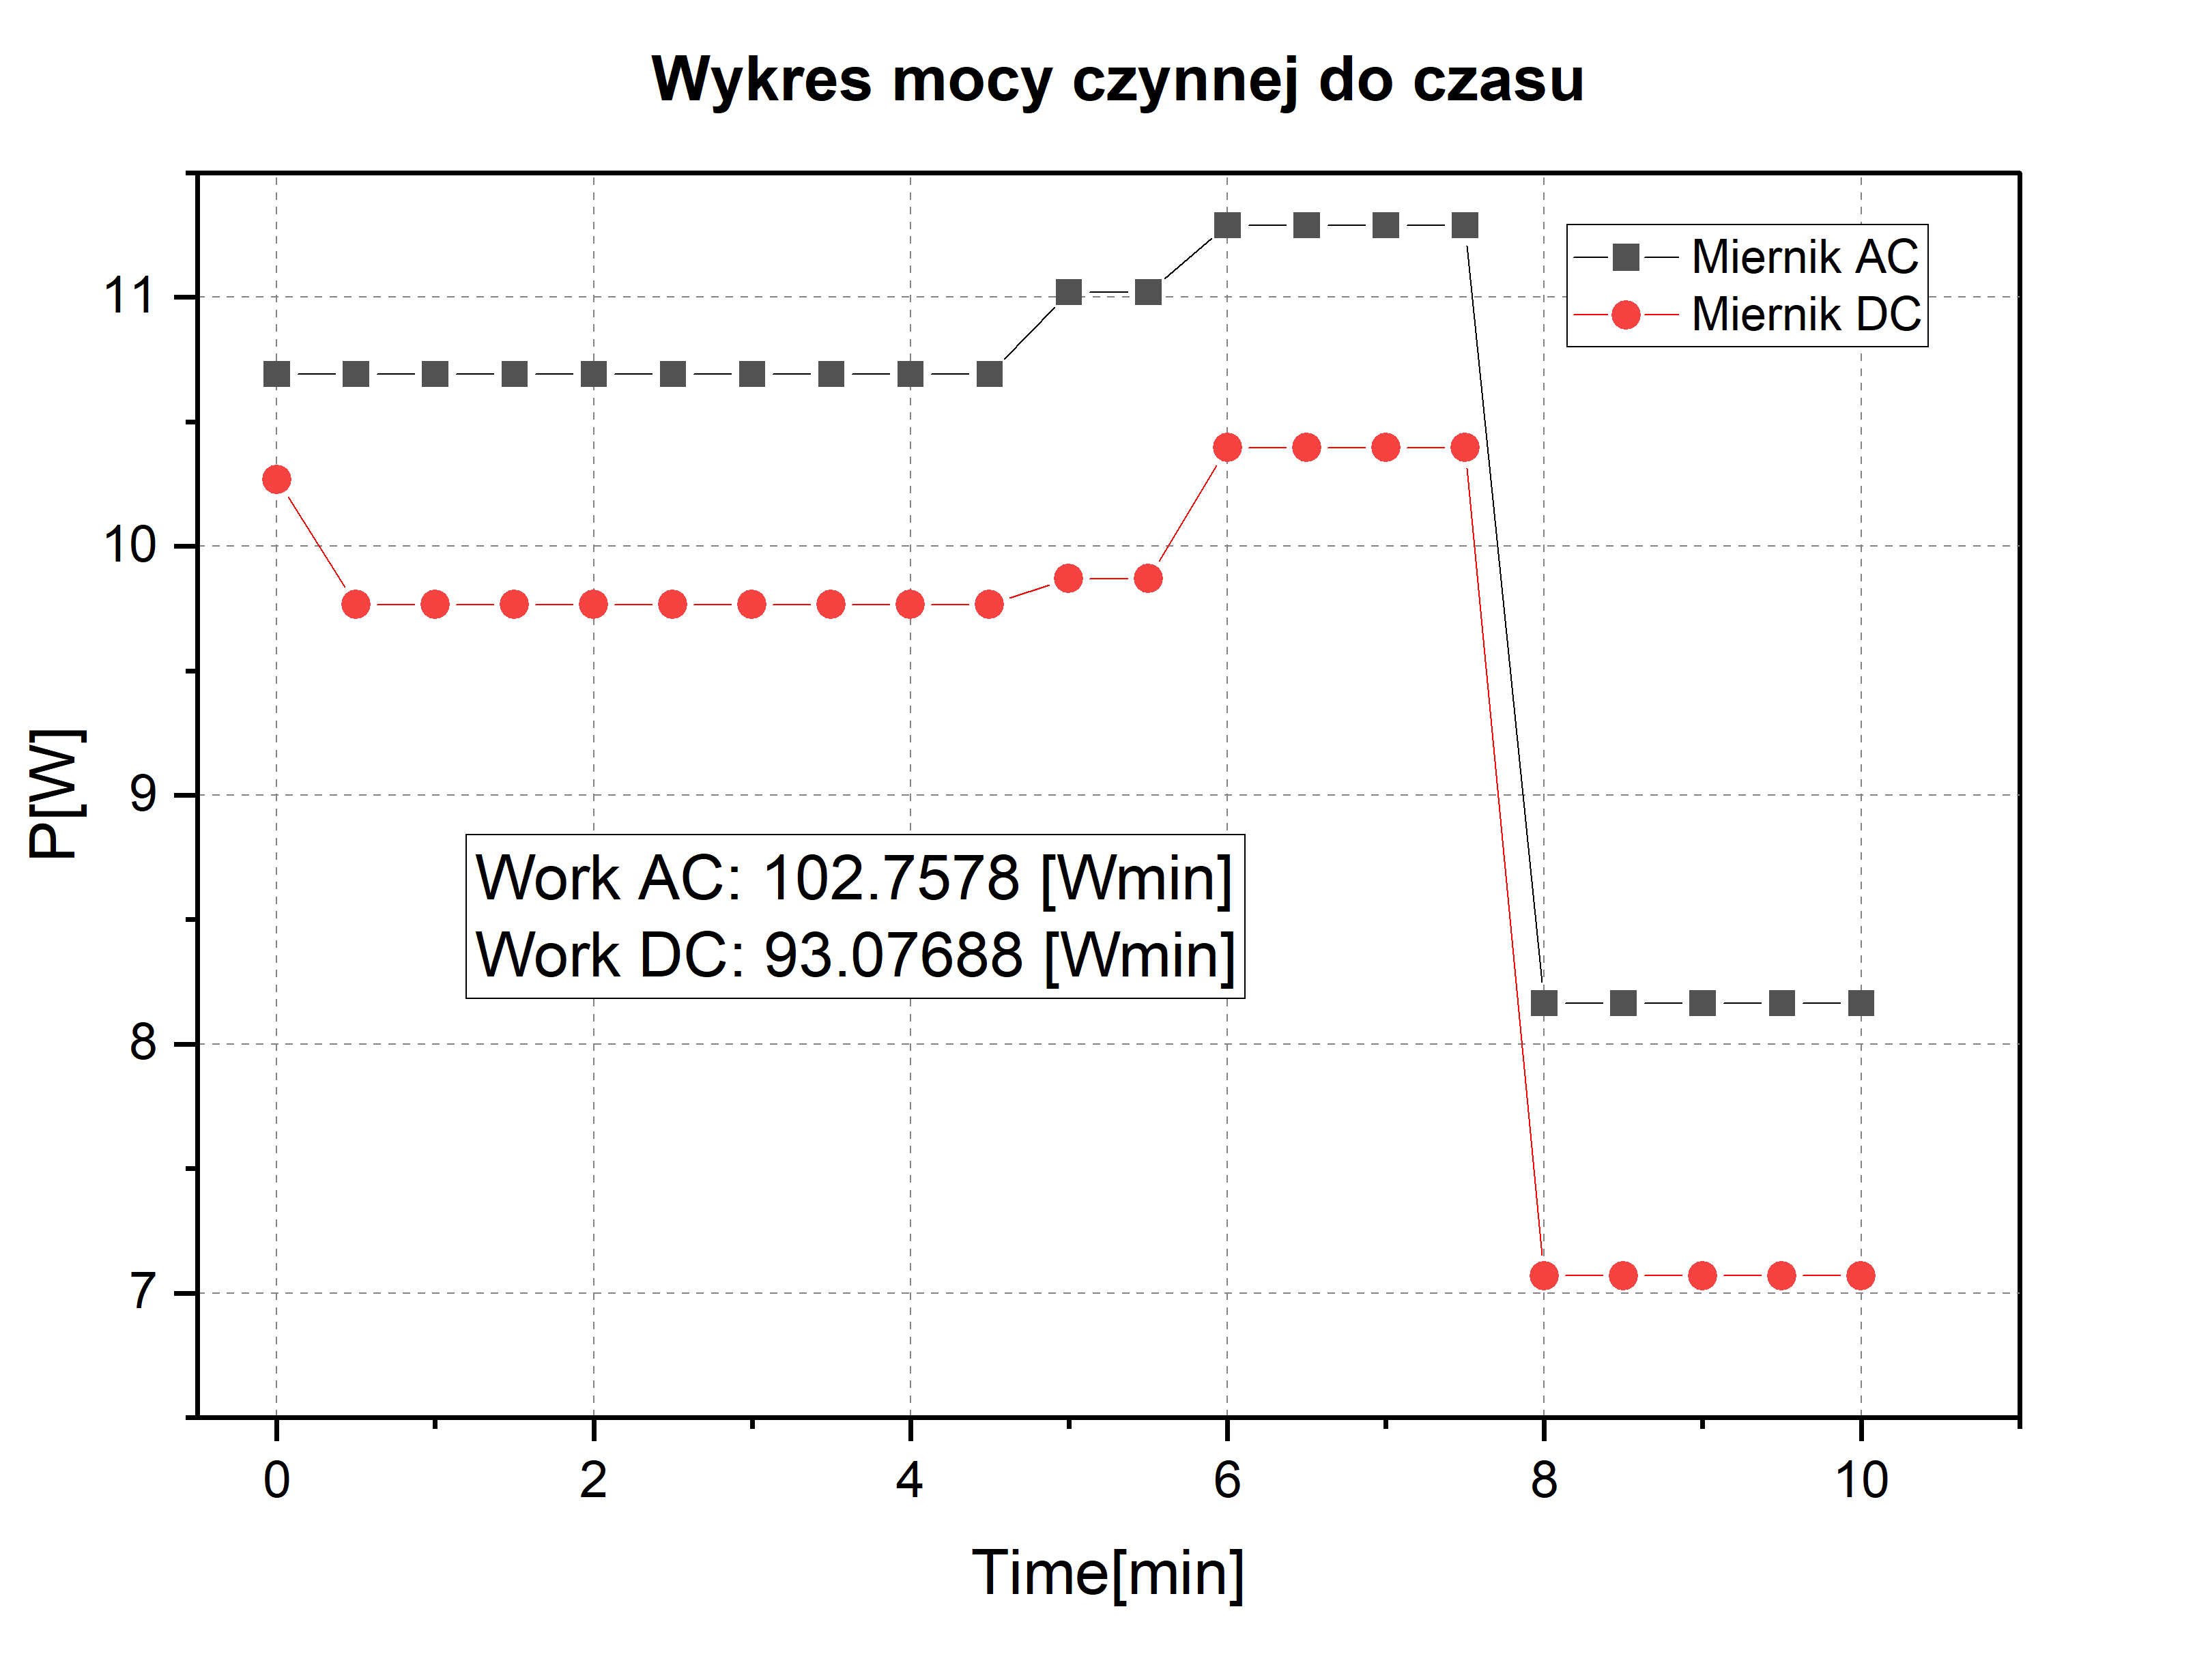
\includegraphics[scale = 0.13]{F:/Projekty Intellij/Text/Metrologia/Ćwiczenie7/Img/origin.png}
    \end{center}
    Energia wyliczona przy pomocy programu OriginPro podana jest w Wato-minutach. Wartości te zostały zamienione na jednostę [Wh] przy pomocy poniższego
    wzoru:
    \begin{gather*}
        P_{Wh}=P_{Wmin}\cdot \frac{1}{60}
    \end{gather*}
    \noindent Przykładowo dla wyniku energii miernika prądu przemiennego dla urządzenia Realme:
    \begin{gather*}
        P_{Wh}=102.7578\cdot \frac{1}{60}=1.712630003[Wh]
    \end{gather*}
    \newpage
    \indent Poniżej została przedstawiona tabela wyników energii zmierzonych przez oba mierniki dla wszystkich urządzeń:
    \begin{center}
        \csvreader[tabular = |c|c|c|,
            table head = \hline  \textbf{Urządzenie} & \textbf{Energia AC[Wh]} & \textbf{Energia DC[Wh]}  \\\hline,
            late after line = \\\hline
        ]{Dane/Wyniki1.csv}{}{
            \csvcoli & \csvcolii & \csvcoliii
        }
    \end{center}
%    TODO: wyjaśnić wyniki
    \par Z powyższych wyników możemy zauważyć, że energia na wejściu ładowarki była większa niż energia na wyjściu. Wynika to z tego
    że część energii pobranej przez ładowarki zamieniona została na straty w postaci np. energii termicznej.

    \subsection*{Część 1 - koszt naładowania}
    Energię wymaganą do pełnego naładowania urządzenia wyliczono z poniższego wzoru:
    \begin{gather*}
        E=\frac{E_x}{L}\cdot 100\%
    \end{gather*}
    {\footnotesize
        \begin{itemize}
            \setlength\itemsep{0em}
            \item[] \textbf{$E_x$} - energia poobrana do naładowania L procent baterii,
            \item[] \textbf{L} - poziom naładownej energii w procentach (różnica między poziomem baterii na końcu i na początku doświadczenia),
        \end{itemize}}
    \noindent Przykładowo dla urządzenia Realme:
    \begin{gather*}
        E=\frac{1.712630003[Wh]}{14\%}\cdot 100\%=12.23307145[Wh]
    \end{gather*}
    \noindent Koszt za moc czynną potrzebną do naładowania w pełni urządzenia wyliczany jest ze wzoru:
    \begin{gather*}
        C_P=\frac{E_{Wh}}{1000}*C_{kWh}
    \end{gather*}
    {\footnotesize
        \begin{itemize}
            \setlength\itemsep{0em}
            \item[] \textbf{$C_P$} - cena za moc czynną,
            \item[] \textbf{$E_{Wh}$} - energia pobrana przez odbiornik w [Wh],
            \item[] \textbf{$C_{kWh}$} - cena 1 [kWh] równa 1.12[PLN]\footnote{Średni koszt 1[kWh] energii elektrycznej dla taryfy G11 dla zużycia 200 kWh/miesiąc we Wrocławiu. Dane aktualne na styczeń 2024r zaczerpnięte z poratalu rachuneo.pl},
        \end{itemize}}
    \noindent Przykładowo dla urządzenia Realme:
    \begin{gather*}
        C_P=\frac{12.23307145[Wh]}{1000}*1.12[\frac{PLN}{kWh}]=0.014[PLN]\approx 0.01[PLN]
    \end{gather*}
    \newpage
    \noindent Moc bierną wyliczamy ze wzoru:
    \begin{gather*}
        Q=U\cdot I\cdot sin(arccos(PF))
    \end{gather*}
    {\footnotesize
        \begin{itemize}
            \setlength\itemsep{0em}
            \item[] \textbf{$PF$} - współczynnik mocy,
        \end{itemize}}
    \noindent Przykładowo dla piątej minuty doświadczenia przy urządzeniu Realme:
    \begin{gather*}
        Q=240[V]\cdot 0.082[A]\cdot sin(arccos(0.56))=16.30[W]
    \end{gather*}
    \indent Wyznaczanie energii mocy biernej potrzebnej do naładowania urządzenia analogiczna do wyznaczania energii mocy czynnej (przy pomocy programu OriginPro i powyższych wzorów).\\
    \indent Koszt energii biernej został wyznaczony z tego samego wzoru co koszt energii czynnej lecz dodatkowo koszt został na końcu przemnożony przez 3.\\
    Poniżej została przedstawiona tabela wyników energii czynnej i biernej potrzebnych do naładowania urządzenia w pełni oraz ceny naładowania urządzenia za moc czynną oraz bierną:
    \begin{center}
        \csvreader[tabular = |c|c|c|c|c|,
            table head = \hline  \textbf{Urządzenie} & \textbf{$E_P$[Wh]} & \textbf{$E_Q$[Wh]}
            & \textbf{Cena$_P$[PLN]} & \textbf{Cena$_Q$[PLN]}  \\\hline,
            late after line = \\\hline
        ]{Dane/Wyniki2.csv}{}{
            \csvcoli & \csvcolii & \csvcoliii & \csvcoliv & \csvcolv
        }
    \end{center}
    \indent Koszt energii został zaokrąglony do dwóch miejsc znaczących gdyż przy zaokrągleniu do jednego grosza stracono by dokładność wyników.
    \newpage
    \subsection*{Część 2 - zasilacz laboratoryjny}
    Poniżej została przedstawiona charakterystyka zależności obciążenia od współczynnika mocy:
    \begin{center}
        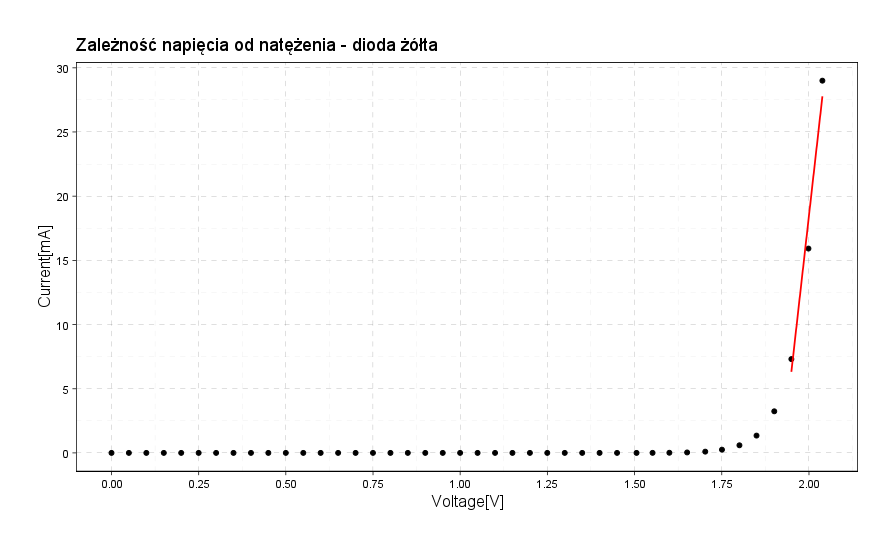
\includegraphics[scale = 0.45]{F:/Projekty Intellij/Text/Metrologia/Ćwiczenie7/Img/Rplot01.png}
    \end{center}
%    TODO: wnioski z charakterystyki
    \par Na podstawie charakterystyki możemy zauważyć, że wraz ze wzrostem obciążenia współczynnik mocy rośnie. Obciążenie na wyjściu zasilacza jest czysto
    rezystancyjne więc samo w sobie miałoby współczynnik mocy równy 1. Oznacza to że współczynnik mocy wynika tylko i wyłącznie z elementów wewnętrznych
    zasilacza. Tego typu zasilacze przeważnie składają się z transformatora który obniża znacząco napięcie sieciowe a po wyprostowaniu napięcia dalsza
    regulacja odbywa się za pomocą przetwornic impulsowych. Tranforormatory dodają bardzo duże przesunięcie fazowe indukcyjne do przebiegu. Na wykresie
    możemy zauważyć kilka charakterystycznych punktów, w których wartości zmieniają się skokowo o dużą wartość.\\
    \indent W trakcie operowania zasilacza również słyszano charakterystyczne "klikanie" \newline przekaźników przy zmianie zakresów na wyższe. Mogłoby to oznaczać że zasilacz posiada kilka odczepów na
    uzwojeniu wtórnym transformatora a sam zasilacz wraz ze wzrostem napięcia wyjściowego przełącza, z którego odczepu podaje napięcie na wyjście.
    Im mniejsze napięcie chcemy uzyskać tym większa przekładnia transformatora i jednocześnie większe przesunięcie fazowe na wejściu. Tłumaczyłoby to
    zachowanie współczynnika mocy wraz ze wzrostem obciążenia.\\
    \\
    \noindent Energię rozproszoną na rezystorze w czasie 1 [h] wyliczamy ze wzoru:
    \begin{gather*}
        E_{dc}=U\cdot I\cdot T
    \end{gather*}
    \noindent Przykładowo dla napięcia 4 [V]:
    \begin{gather*}
        E_{dc}=4[V]\cdot 1.71[A]\cdot 1[h]=6.84[Wh]
    \end{gather*}
    \indent Koszt energii pobranej przez zasilacz wyliczamy tak jak w poprzedniej części ćwiczenia.\\
    Poniżej przedstawiono tabelę przedstawiającą energię pobraną przez zasilacz, energię rozproszoną na rezystorze oraz koszt
    energii pobranej przez zasilacz w czasie 1 [h] dla każdego napięcia:
    \begin{center}
        \csvreader[tabular = |c|c|c|c|,
            table head = \hline  \textbf{U[V]} & \textbf{$E_{rez}$[Wh]} & \textbf{$E_{zas}$[Wh]} & \textbf{Koszt[PLN]} \\\hline,
            late after line = \\\hline
        ]{Dane/Wyniki3.csv}{}{
            \csvcoli & \csvcolii & \csvcoliii & \csvcoliv
        }
    \end{center}

    \subsection*{Część 3 - pobór mocy i współczynnik mocy dla różnych urządzeń}
    \noindnet Wszystkie obliczenia tak jak w poprzednich częściach.
    \begin{center}
        \csvreader[tabular = |c|c|c|c|c|,
            table head = \hline  \textbf{Urządzenie} & \textbf{$E_P$[Wh]} & \textbf{Koszt$_P$[PLN]}
            & \textbf{$E_Q$[Wh]} & \textbf{Koszt$_Q$[PLN]}  \\\hline,
            late after line = \\\hline
        ]{Dane/Wyniki4.csv}{}{
            \csvcoli & \csvcolii & \csvcoliii & \csvcoliv & \csvcolv
        }
    \end{center}

    \section{Uwagi i wnioski}
    Z części 1 możemy wyciągnąć wiele interesujących wniosków. Zauważamy że niektóre ładowarki dostosowują napięcie ładowania do poziomu naładowania akumulatora podczas
    gdy prostsze konstrukcje ładują stałym napięciem i prądem. Empirycznie możemy też zauważyć straty energi w procesie zmiany napięcia sieciowego na stałe napęcie ładowania.
    Również zauważamy jak duży wkład w moc pozorną ma moc bierna, która dla wszystkich trzech ładowarek była większa niż moc czynna.\\
    \newpage
    \indent Z części 2 udało się wyznaczyć charakterystykę współczynnika mocy od obciążenia i określić jaki charakter może mieć obciążenie na podstawie zmian współczynnika mocy wraz ze wzrostem
    napięcia na wyjściu zasilacza.\\
    \\
    \indent  W części 3 wyznaczono energię czynną oraz bierna pobraną przez typowe urządzenia domowe w ciągu doby oraz koszt tej energii. Można zauważyć że urządzenia czysto rezystancyjne
    takie jak czajnik nie pobierają mocy biernej w czasie swojej operacji. Jednocześnie większość urządzeń czysto rezystancyjnych wykorzystywana jest do wytwarzania energii cieplenj
    np. czajniki, kuchenki oporowe, grzejniki elektryczne. Urzadzenia te pobierają ogromne ilości energi elektrycznej a koszt ich zasilenia jest jednym z głownych kosztów energii
    elektrycznej w domach rodzinnych. Możemy zauważyć też w przypadku np. niszczarki że koszt mocy biernej w tym przypadku potrafił zrównać się z kosztem mocy czynnej. Na szczęście
    jako domy rodzinne nie płacimy za moc bierną i całe szczęście gdyż mogłoby to znacząco podnieść koszty energii elektrycznej.\\
    \indent Warto jednak zaznaczyć że duże zakłady/fabryki muszą brać pod uwagę może nie sam współczynnik moc, ale przesunięcie fazowe generowane przez urządzenia znajdujące się
    na terenie zakładu. Nie dość że firmy te płacą za przesunięcie fazowe w sieci spowodowane przez ich zakład to dodatkowo przesunięcie fazowe źle wpływa na wiele urzadzeń
    takich zakładach. Muszą się oni liczyć więc z kompensowaniem przesunięcia fazowego przy pomocy np. banków kondensatorów (gdyż często przesunięcie fazowe wynika głownie z silników
    indukcyjnych, transformatorów - które powodują przesunięcie indukcyjne).

%Bibliografia
    \vfill
    \footnotesize
    \begin{thebibliography}{9}
        \bibitem{texbook1}
        https://wzn.pwr.edu.pl/materialy-dydaktyczne/metrologia-elektroniczna
    \end{thebibliography}

\end{document}